\chapter{Graphics Processing Units}\label{chapter:graphics_processing_units}

In this work, we aim to accelerate the execution of our solver using a relatively new architecture,
\acrshortpl{acr:GPU}. \Acrshortpl{acr:GPU} are massively parallel computer chips that have recently
started to be used in the scientific computing domain. \Acrshortpl{acr:GPU} were initially designed
to perform repetitive graphical computations, such as the output to a computer screen, video
processing, and synthetic image generation. These computations are \textit{embarrassingly parallel},
meaning that they are comprised of many identical computations independent of each other.
\Acrshortpl{acr:GPU} are therefore optimised for parallel efficiency. Since these problems deal with
huge amounts of data, \acrshortpl{acr:GPU} are also optimised for maximum bandwidth. They are
significantly different from \textit{\acrfullpl{acr:CPU}}, the traditional architecture on which
code is run. \Acrshortpl{acr:CPU} are optimised to solve serial problems as fast as possible,
meaning they prioritise serial speed over parallel efficiency, and latency over bandwidth. 

Solving fluid flows on a mesh is a parallel problem, as at most steps it is possible to compute the
solution on the different elements making up the mesh in parallel. On the other hand, elements must
exchange information at their interfaces at each time step, meaning careful synchronisation will be
needed. Finally, the \acrlong{acr:AMR} process detailed in
Chapter~\ref{chapter:adaptive_mesh_refinement} and the dynamic load balancing process from
Chapter~\ref{chapter:load_balancing} are not inherently parallel processes. A significant
programming effort then becomes necessary to break up these algorithms into parallel tasks to be run
on \acrshortpl{acr:GPU}. Overall, if it is possible to efficiently parallelise these sequential
parts of the problem, the gains from running the main solving loop on the highly parallel
\acrshortpl{acr:GPU} should incur a significant speedup to the program.

\section{Architecture}\label{section:graphics_processing_units:architecture}

\subsection{Hardware model}\label{subsection:graphics_processing_units:architecture:hardware_model}

\Acrlongpl{acr:GPU} and \acrlongpl{acr:CPU} are fundamentally made up of the same core components.
First, data processing hardware, shown in green in Figure~\ref{fig:cpu_gpu}, consists of the parts
of the chips that do calculations on data. Control flow hardware, shown in yellow, schedules
instructions to be executed on processing hardware. In orange is the main memory of either
architecture. Main memory or \textit{\acrfull{acr:DRAM}}, shown in orange, stores data to be used
for computations. The main memory is very big, and takes a relatively long time to access. Finally,
in blue and purple are different levels of cache memory. Cache is much smaller and much faster than
main memory, and as such stores parts of the memory that the processing hardware is actively using
in order to speed up access.

\begin{figure}[H]
    \centering
    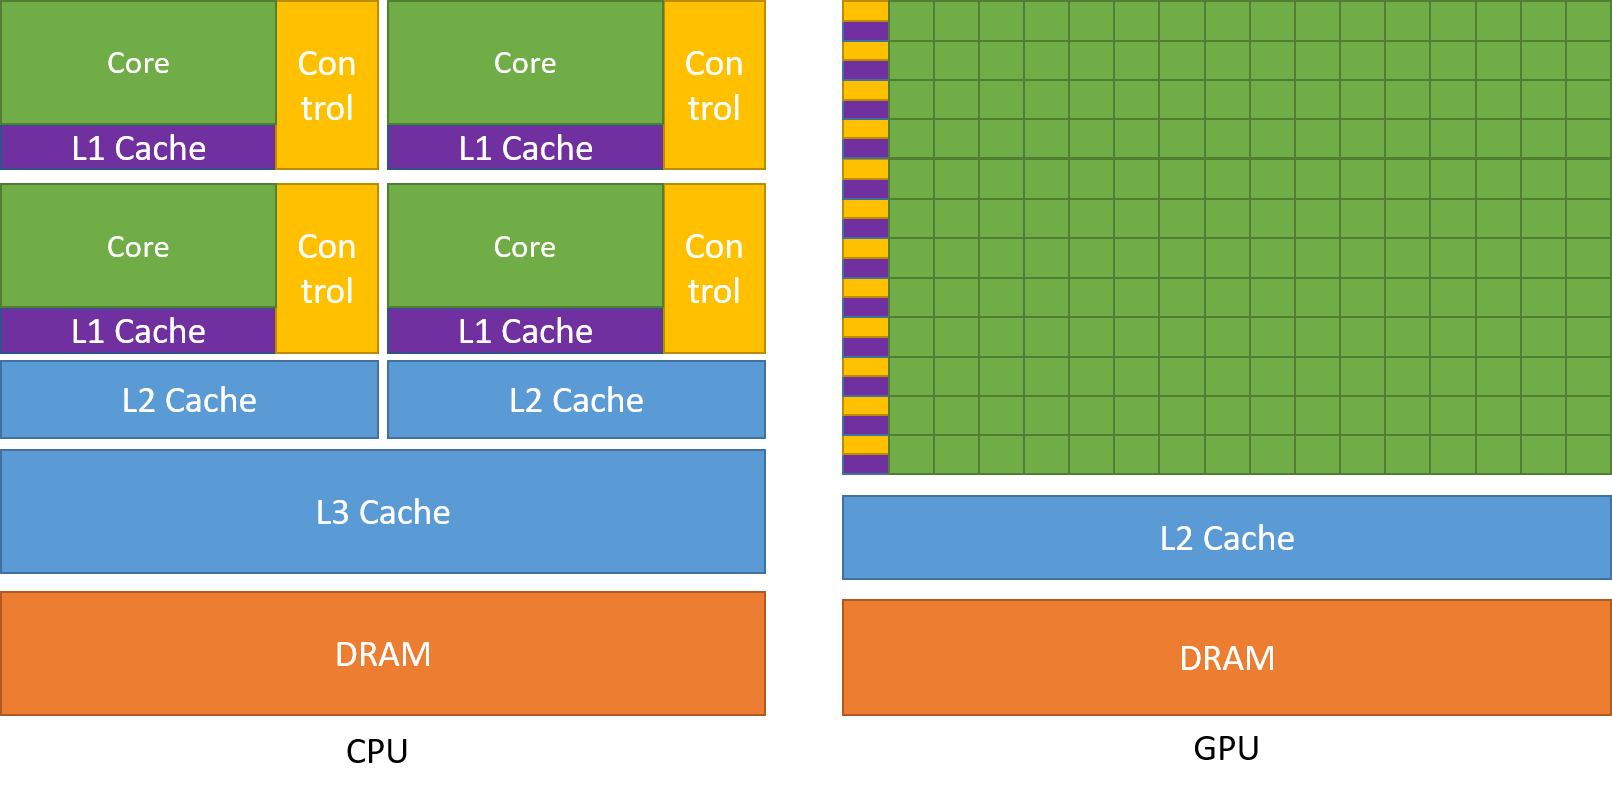
\includegraphics[width=0.8\textwidth]{Chapter_graphics_processing_units/media/gpu-devotes-more-transistors-to-data-processing}
    \caption{\Acrshort{acr:CPU} and \acrshort{acr:GPU} architecture~\cite{Nvidia2021}: \acrshortpl{acr:GPU} dedicate more space to data processing}\label{fig:cpu_gpu}
\end{figure}

The two architectures differ in the balance between the size and capacities of these components.
Chip area is limited by the processes used to manufacture them, so the different components must
share this limited space, and sacrifices must be made. \Acrshortpl{acr:GPU} dedicate much more space
to data processing, increasing throughput. Their compute units are also smaller, to work on more
data in parallel. \Acrshortpl{acr:CPU}, on the other hand, have fewer bigger compute units with a
higher clock speed in order to reduce latency. Their compute units are called cores. The
\acrshort{acr:GPU} compute units are called \acrshort{acr:CUDA} cores, and are arranged in rows as
\textit{\acrfullpl{acr:SM}}.

In order to reduce latency, \acrshortpl{acr:CPU} have a lot of die space dedicated to cache. More
cache helps keep data close in access time. More data is loaded from main memory at a time, assuming
that data that is near needed data will also be needed later. The deeper hierarchy of cache of
\acrshortpl{acr:CPU} helps keep the cores working on the current problem as fast as possible, never
starving for memory. \Acrshortpl{acr:GPU} have less total cache and fewer levels of cache to make
room for more \acrshort{acr:CUDA} cores. As a throughput oriented device, it is less important how
fast individual tasks complete, as long as more tasks overall are completed. The reduced cache is
acceptable because if a \acrshort{acr:CUDA} core is waiting on data from the main memory that was
not found in cache, it will simply pause execution of that thread and execute another thread. On
\acrshortpl{acr:GPU}, the smallest and fastest cache, L1 cache, is shared within a
\acrshort{acr:SM}. Accessing shared data is therefore fast as long as conflicts are avoided.

Finally, \acrshortpl{acr:CPU} also reduce latency by using much more potent control flow units.
Firstly, they have one control flow unit per core, where \acrshortpl{acr:GPU} have one control flow
unit per row of cores. This limits how many instructions can be dispatched to the cores making up a
\acrshort{acr:SM}. The cores will therefore execute the same instruction at the same time in groups
of 32, called warps. This makes branching much more expensive if it happens within a warp. If a part
of a program has two branches, A and B, the cores executing branch A will go first, followed by the
cores executing branch B. These have to be executed sequentially because the control flow unit can
only dispatch one instruction per warp. This multiplies the computation time by the number of taken
branches. \Acrshort{acr:CPU} cores only execute a single branch, or can even execute both branches
at once while waiting for the result of the conditional, keeping only the correct result once the
conditional has been evaluated. The more powerful control flow units of \acrshortpl{acr:CPU} may
also perform branch prediction, consisting of the \acrshort{acr:CPU} guessing the most likely branch
based on the result of previous computations and starting to execute this branch while waiting for
the conditional. All this is performed in an effort to reduce latency as much as possible. Programs
running on \acrshortpl{acr:GPU} must compensate by avoiding divergence as much as possible within
warps.

\subsection{Programming model}\label{subsection:graphics_processing_units:architecture:programming_model}

This work uses the \acrshort{acr:CUDA} programming model. It is a programming language, framework
and runtime \acrfull{acr:API} developed to enable programming on \acrshortpl{acr:GPU} with an
extension of the C++ language. Programs using the language execute on the \acrshort{acr:CPU} like
normal programs, but can schedule parts of the program, called kernels, to be executed on the
\acrshort{acr:GPU}. Kernels are run in parallel on the \acrshort{acr:GPU}, asynchronously from the
\acrshort{acr:CPU}. The \acrshort{acr:CPU} is therefore free to do computations of its own while the
\acrshort{acr:GPU} is executing, including adding more kernels or transfers to the
\acrshort{acr:GPU} execution queue. Multiple such queues, called streams, can exist. The purpose of
using multiple streams is to execute independent computations on the \acrshort{acr:GPU}
concurrently, and maximise \acrshort{acr:GPU} usage in case a stream is waiting.
\Acrshortpl{acr:GPU} can concurrently execute kernels, transfer data from the \acrshort{acr:CPU} to
the \acrshort{acr:GPU}, and transfer data from the \acrshort{acr:GPU} to the \acrshort{acr:CPU}.
These transfers are necessary because \acrshort{acr:CPU} and \acrshort{acr:GPU} main
\acrlong{acr:RAM} are separate. Data needed for computations on the \acrshort{acr:GPU} that cannot
be generated on it must be explicitly transferred from the \acrshort{acr:CPU}, and results living on
the \acrshort{acr:GPU} must be transferred back to the \acrshort{acr:CPU} in order to be displayed
or written to disk. As \acrshortpl{acr:GPU} are also generally running the displays of non-server
computers, results that are only meant to be viewed can be directly displayed and such transfers can
be skipped. This is not the case for this work. 

\begin{figure}[H]
    \centering
    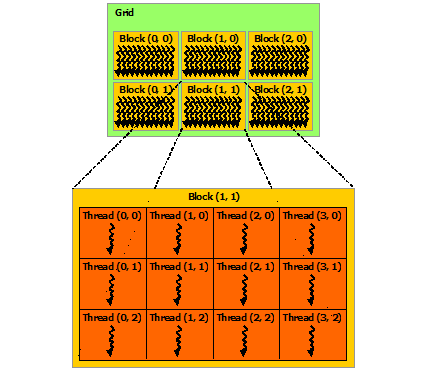
\includegraphics[width=0.6\textwidth]{Chapter_graphics_processing_units/media/grid-of-thread-blocks}
    \caption{\Acrshort{acr:GPU} programming model~\cite{Nvidia2021}: Execution is split into multiple parallelism levels}\label{fig:gpu_programming_model}
\end{figure}

The programing model ties in with the hardware model from
Subsection~\ref{subsection:graphics_processing_units:architecture:hardware_model} by decomposing the
execution of kernels to multiple parallel levels. A kernel will be executed in parallel, with each
core executing the same function. Figure~\ref{fig:gpu_programming_model} shows how the programming
model decomposes a problem. The whole problem to be solved is represented as a multidimensional grid
of tasks, with two dimensions in this example. The kernel will execute until the whole grid has been
computed. The grid is broken up into blocks of threads. The different blocks will be dispatched to
the \acrlongpl{acr:SM} of the \acrshort{acr:GPU}, and each thread of that block will be executed on
a \acrshort{acr:CUDA} core of the \acrshort{acr:SM}. A \acrshort{acr:SM} can execute multiple blocks
at the same time if there are more cores within the \acrshort{acr:SM} than threads within a block.
Blocks need to be completely independent of each other, as they cannot be synchronised and may
execute in any order. They also cannot share local memory, as each \acrshort{acr:SM} has its own L1
cache. Threads within the same block can depend on one another, as they are executed concurrently on
the same \acrshort{acr:SM}. Threads from a block execute the same instruction at the same time in
groups of 32, or warps. This is the \textit{\acrfull{acr:SIMT}} architecture. If there are more
threads within a block than cores within a \acrshort{acr:SM}, warps will be run sequentially until
all threads are done with the instruction. Threads within a block can share local memory, and
synchronise with each other. This is useful for algorithms with steps like reductions, where threads
will wait until all threads have computed one level of the reduction, to use the result of that
level for the next one.

Typical execution of a program that adds an array A to an array B and stores the result in an array
C will proceed as follows. The \acrshort{acr:CPU} side of the program will create two arrays of data
in its memory, and initialise them as needed. It will then create two arrays of the same size on the
\acrshort{acr:GPU} using the \acrshort{acr:CUDA} runtime \acrshort{acr:API}, and transfer the data
from the \acrshort{acr:CPU} arrays A and B to the \acrshort{acr:GPU} arrays. It will then create a
result array C on the \acrshort{acr:GPU}, and one on the \acrshort{acr:CPU}. It will then launch a
kernel on the \acrshort{acr:GPU}, with pointers to the \acrshort{acr:GPU} A and B arrays, and the
\acrshort{acr:GPU} C array. The number of elements in the vectors will dictate the size of the
execution grid. The number of elements will be split in blocks of threads of fixed size, for example
blocks of 128 threads. The number and size of blocks are given to the \acrshort{acr:GPU} when
calling the kernel. The \acrshort{acr:CPU} then must wait until the computation is done using a
synchronisation with the \acrshort{acr:CUDA} runtime, transfer the data from the \acrshort{acr:GPU}
C array to the \acrshort{acr:CPU} C array, and display the results. 

This model fits well with many \acrshort{acr:CFD} methods, including the \acrshort{acr:DG-SEM} used
in this work. We work on a mesh made up of elements and faces connecting them. Elements are
independent during most of the computation and their computations can be executed in parallel. The
only step from the main solver loop needing extra care is the computation of the fluxes between the
elements. The flux computation needs the data from the elements on either side of a face and stores
the resulting flux back in both elements so they can compute their derivative. Since there can be
multiple faces on each side of an element as detailed in
Section~\ref{section:adaptive_mesh_refinement:mortar_element_method}, and each element has multiple
sides, multiple threads will attempt to read and write to the same locations at the same time. This
is a race condition, where the result of the computation will depend on the order in which the
threads try to access the memory location. The results may also be wrong. If two threads read a
value, add their contribution, and store the value, only whichever thread wrote its result last will
have its contribution accounted for in the final result. Different approaches are possible to solve
this issue. For example, Giuliani and Krivodonova~\cite{Giuliani2019} use an edge colouring method
where the same kernel is run multiple times on different edges in order to avoid writing to the
elements at the same time. Our program parallelises this part of the computation on the faces
connecting the elements instead, as described in
Section~\ref{section:spectral_element_method:implementation}. As long as there are enough elements
in the mesh to saturate the cores of the \acrshort{acr:GPU} with work, this part of the program
should be efficient to run on the \acrshort{acr:GPU}.

The \acrlong{acr:AMR} and dynamic load balancing algorithms shown in
Chapters~\ref{chapter:adaptive_mesh_refinement} and~\ref{chapter:load_balancing} are not so easily
parallelised. These algorithms are sequential in nature, with many operations needing the result of
previous ones to complete their calculations. In order to parallelise them, a few support structures
have to be added for the different processing threads to be able to find the data they have been
assigned, and the different memory locations they are allowed to access. In addition, a kernel
operating on certain objects, elements for example, should not modify other objects, such as faces.
This is done to avoid race conditions when multiple threads try to access the same memory location,
faces in this example. The practical consequence of this is that objects moving to a new index in
their storage arrays cannot update their neighbour faces to point to their new index. Their
neighbours must therefore have the required information to compute where the element will move when
the face moves itself, and update the index itself. By designing the algorithms this way, a kernel
running on an object type will have each thread writing to only a single object corresponding to its
index, avoiding race conditions. More information on how the algorithms are designed is available in
Sections~\ref{section:spectral_element_method:implementation},~\ref{section:adaptive_mesh_refinement:implementation}
and~\ref{section:load_balancing:implementation}.

The meshes generated by \acrlong{acr:AMR} and dynamic load balancing are also not naturally suited
for \acrshortpl{acr:GPU}. These processors are more suited for static repetitive tasks. Element
splitting, changing their polynomial order and moving elements around will reduce the efficiency of
the computations if care is not taken to tune the algorithms to this platform. Elements with
different polynomial orders in a thread warp will introduce branching, and the warp will take as
much time to execute as the highest polynomial order elements. Moving and splitting elements will
put more pressure on the limited cache of \acrshortpl{acr:GPU}, as threads will loop over different
elements after refinement and load balancing. The interval between each refinement and load
balancing will have to be tuned to trade off between having an optimal mesh for computations and
having a static mesh for more iterations.

\section{Process Parallelism}\label{section:graphics_processing_units:process_parallelism}

When trying to solve very large problems, a single node with a single \acrshort{acr:GPU} will have
insufficient processing power and memory to solve the problem in a reasonable amount of time, or at
all. To work with these larger problems, the work needs to be split at another level than
\acrshort{acr:GPU} parallelism.  

The program can use multi-block meshes, with each block being worked on by one process and one
\acrshort{acr:GPU}. If there are fewer \acrshortpl{acr:GPU} available on a system than there are
processes, some processes will share a single \acrshort{acr:GPU} by using asynchronous execution
streams. The different processes communicate together using \textit{\acrfull{acr:MPI}} at their
boundaries. Since the solution data resides on the \acrshort{acr:GPU}, it must first be copied to
the main \acrshort{acr:CPU} memory before it is sent through the \acrshort{acr:MPI} runtime. It then
needs to be copied to the receiving process' \acrshort{acr:GPU}. This exchange necessitates multiple
transfers on different levels and should be optimised as much as possible. An approach to minimise
the number of interfaces between the different mesh blocks is explained in
Section~\ref{section:load_balancing:hilbert_curve}. 

It is possible to split the mesh into more blocks than there are \acrshortpl{acr:GPU} in a system.
In this case, there will be one process per block, and some processes will share
\acrshortpl{acr:GPU}. The \acrshortpl{acr:GPU} will be split into virtual partitions, using
concurrent execution streams. These streams execute concurrently on a \acrshort{acr:GPU}, leveraging
the fact that some operations can happen at the same time. A \acrshort{acr:GPU} can execute up to
one running kernel, one transfer from the \acrshort{acr:CPU} to the \acrshort{acr:GPU}, and one
transfer from the \acrshort{acr:GPU} to the \acrshort{acr:CPU}. Additionally, the \acrshort{acr:GPU}
can execute one kernel while another kernel is waiting for memory. These partitions do not increase
performance, but are useful to test running more blocks than there are available
\acrshortpl{acr:GPU}, or running the program with a mesh that is split into more blocks than
available \acrshortpl{acr:GPU} without re-splitting it.

A simple mesh generator program and a mesh partitioner are available as part of this work. The mesh
generator can create square meshes of arbitrary resolution with different boundary conditions. The
mesh partitioner can split arbitrary single block meshes to multi-block meshes.

These tasks, each consisting of a mesh block, do not necessarily need to run on
\acrshortpl{acr:GPU}. A \acrshort{acr:CPU} version of the program is provided to compare the
efficiency of the program and to aid debugging. That version uses \acrshort{acr:CPU} workers doing
the same computations. The program could even be modified to dispatch work to \acrshort{acr:CPU} and
\acrshort{acr:GPU} workers to use the full computing power of a system. Some work would need to be
done to ascertain the relative capacity of the different workers, as a \acrshort{acr:GPU} worker
running on a complete \acrshort{acr:GPU} is much faster than a \acrshort{acr:CPU} worker running on
a single \acrshort{acr:CPU} core. \Acrshort{acr:CPU} workers could also use multiple threads, with
an architecture similar to the \acrshort{acr:GPU} one.

\section{Data Structure}\label{section:graphics_processing_units:data_structure}

The data structure used in this work has been designed to provide good performance on the
\acrshort{acr:GPU} architecture, while keeping the ease of use and programming of \acrshort{acr:CPU}
code. The mesh is unstructured, made up of elements, faces and nodes.
Figure~\ref{fig:mesh_structure} shows the different components of a two block mesh.

\begin{figure}[H]
    \centering
    \subfloat[First mesh block]
    {\includesvg[height=0.55\textwidth]{Chapter_graphics_processing_units/media/mesh_0_after0_P2_MOD}\label{fig:mesh_left}}
    \hfill
    \subfloat[Second mesh block]
    {\includesvg[height=0.55\textwidth]{Chapter_graphics_processing_units/media/mesh_1_after0_P2}\label{fig:mesh_right}}
    \caption{Data structure: A refined mesh split into two blocks (a) First block (b) Second block}\label{fig:mesh_structure}
\end{figure}

\subsection{Performance}\label{subsection:graphics_processing_units:data_structure:performance}

In order to get good performance and fit naturally with the \acrshort{acr:GPU} architecture, the
different objects are stored as flat one-dimensional arrays on the \acrshort{acr:GPU}. The
\acrshort{acr:CUDA} memory allocation functions are run on the \acrshort{acr:CPU} and return a
continuous block of memory on the \acrshort{acr:GPU}, and the memory transfers between the
\acrshort{acr:CPU} and \acrshort{acr:GPU} copy continuous blocks of memory. This matches well with
having flat arrays of objects. Other data structures, like trees, would need multiple memory
allocations from the \acrshort{acr:CPU} and a kernel to assemble them in some kind of structure.
This would be manageable for a non-adaptive solver as it would be performed once, but with mesh
refinement and load balancing the mesh changes constantly. With arrays, an array of the new size is
allocated and the objects are moved to it. Thanks to the structure from
Subsection~\ref{subsection:graphics_processing_units:data_structure:ease_of_programming}, the
elements themselves have a known constant size regardless of polynomial order, and have the bulk of
their data outside the element object, making them fast to move and making the element array
smaller. The flat arrays also reduce indirection and structure the memory accesses. Memory
indirection occurs when data is not accessed directly, but multiple data structures must be accessed
sequentially to find the address of where the data is stored. Threads from a kernel executing on
elements directly access the element at their thread index in the element array.

This greatly simplifies transfers between the \acrshort{acr:CPU} and \acrshort{acr:GPU}, and mesh
reallocation when refining or load balancing. On the other hand, it carries less context on the
relation between mesh blocks, complicating the element exchanges from the load balancing process of
Chapter~\ref{chapter:load_balancing}. It also means that elements and faces move around in the
arrays as more are added, and their indices must be updated in other objects linking to them. 

Some data needs to be transferred to the \acrshort{acr:CPU} during the computation, such as fluxes
between mesh blocks in different processes, and data to be written to the output files. These
transfers use arrays allocated on the \acrshort{acr:CPU} and \acrshort{acr:GPU}, and a kernel
storing the data into the \acrshort{acr:GPU} array. The array can then be transferred to the
\acrshort{acr:CPU}, and either written to disk or sent to another \acrshort{acr:CPU} and then its
\acrshort{acr:GPU}.

\subsection{Ease of use}\label{subsection:graphics_processing_units:data_structure:ease_of_use}

In order to increase ease of use, the program is made to work with unstructured meshes. Unstructured
meshes allow for increased flexibility when meshing, and an unstructured mesh solver can easily be
made to also read structured meshes. In unstructured meshes, elements are not necessarily numbered
in any order. Elements hold an explicit list of the indices of their neighbours. In structured
meshes, elements are placed in a regular grid, and have an index describing their location. In 2D,
this is the row and column of the element. The neighbours of an element are found by simply
incrementing or decreasing by one the index. Figure~\ref{fig:mesh_types} shows a comparison of the
two types of meshes used to represent the same geometry. 

\begin{figure}[H]
    \centering
    \subfloat[Structured mesh]
    {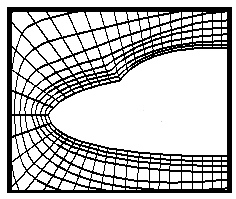
\includegraphics[width=0.45\textwidth]{Chapter_graphics_processing_units/media/structured_mesh}\label{fig:structured_mesh}}
    \qquad
    \subfloat[Unstructured mesh]
    {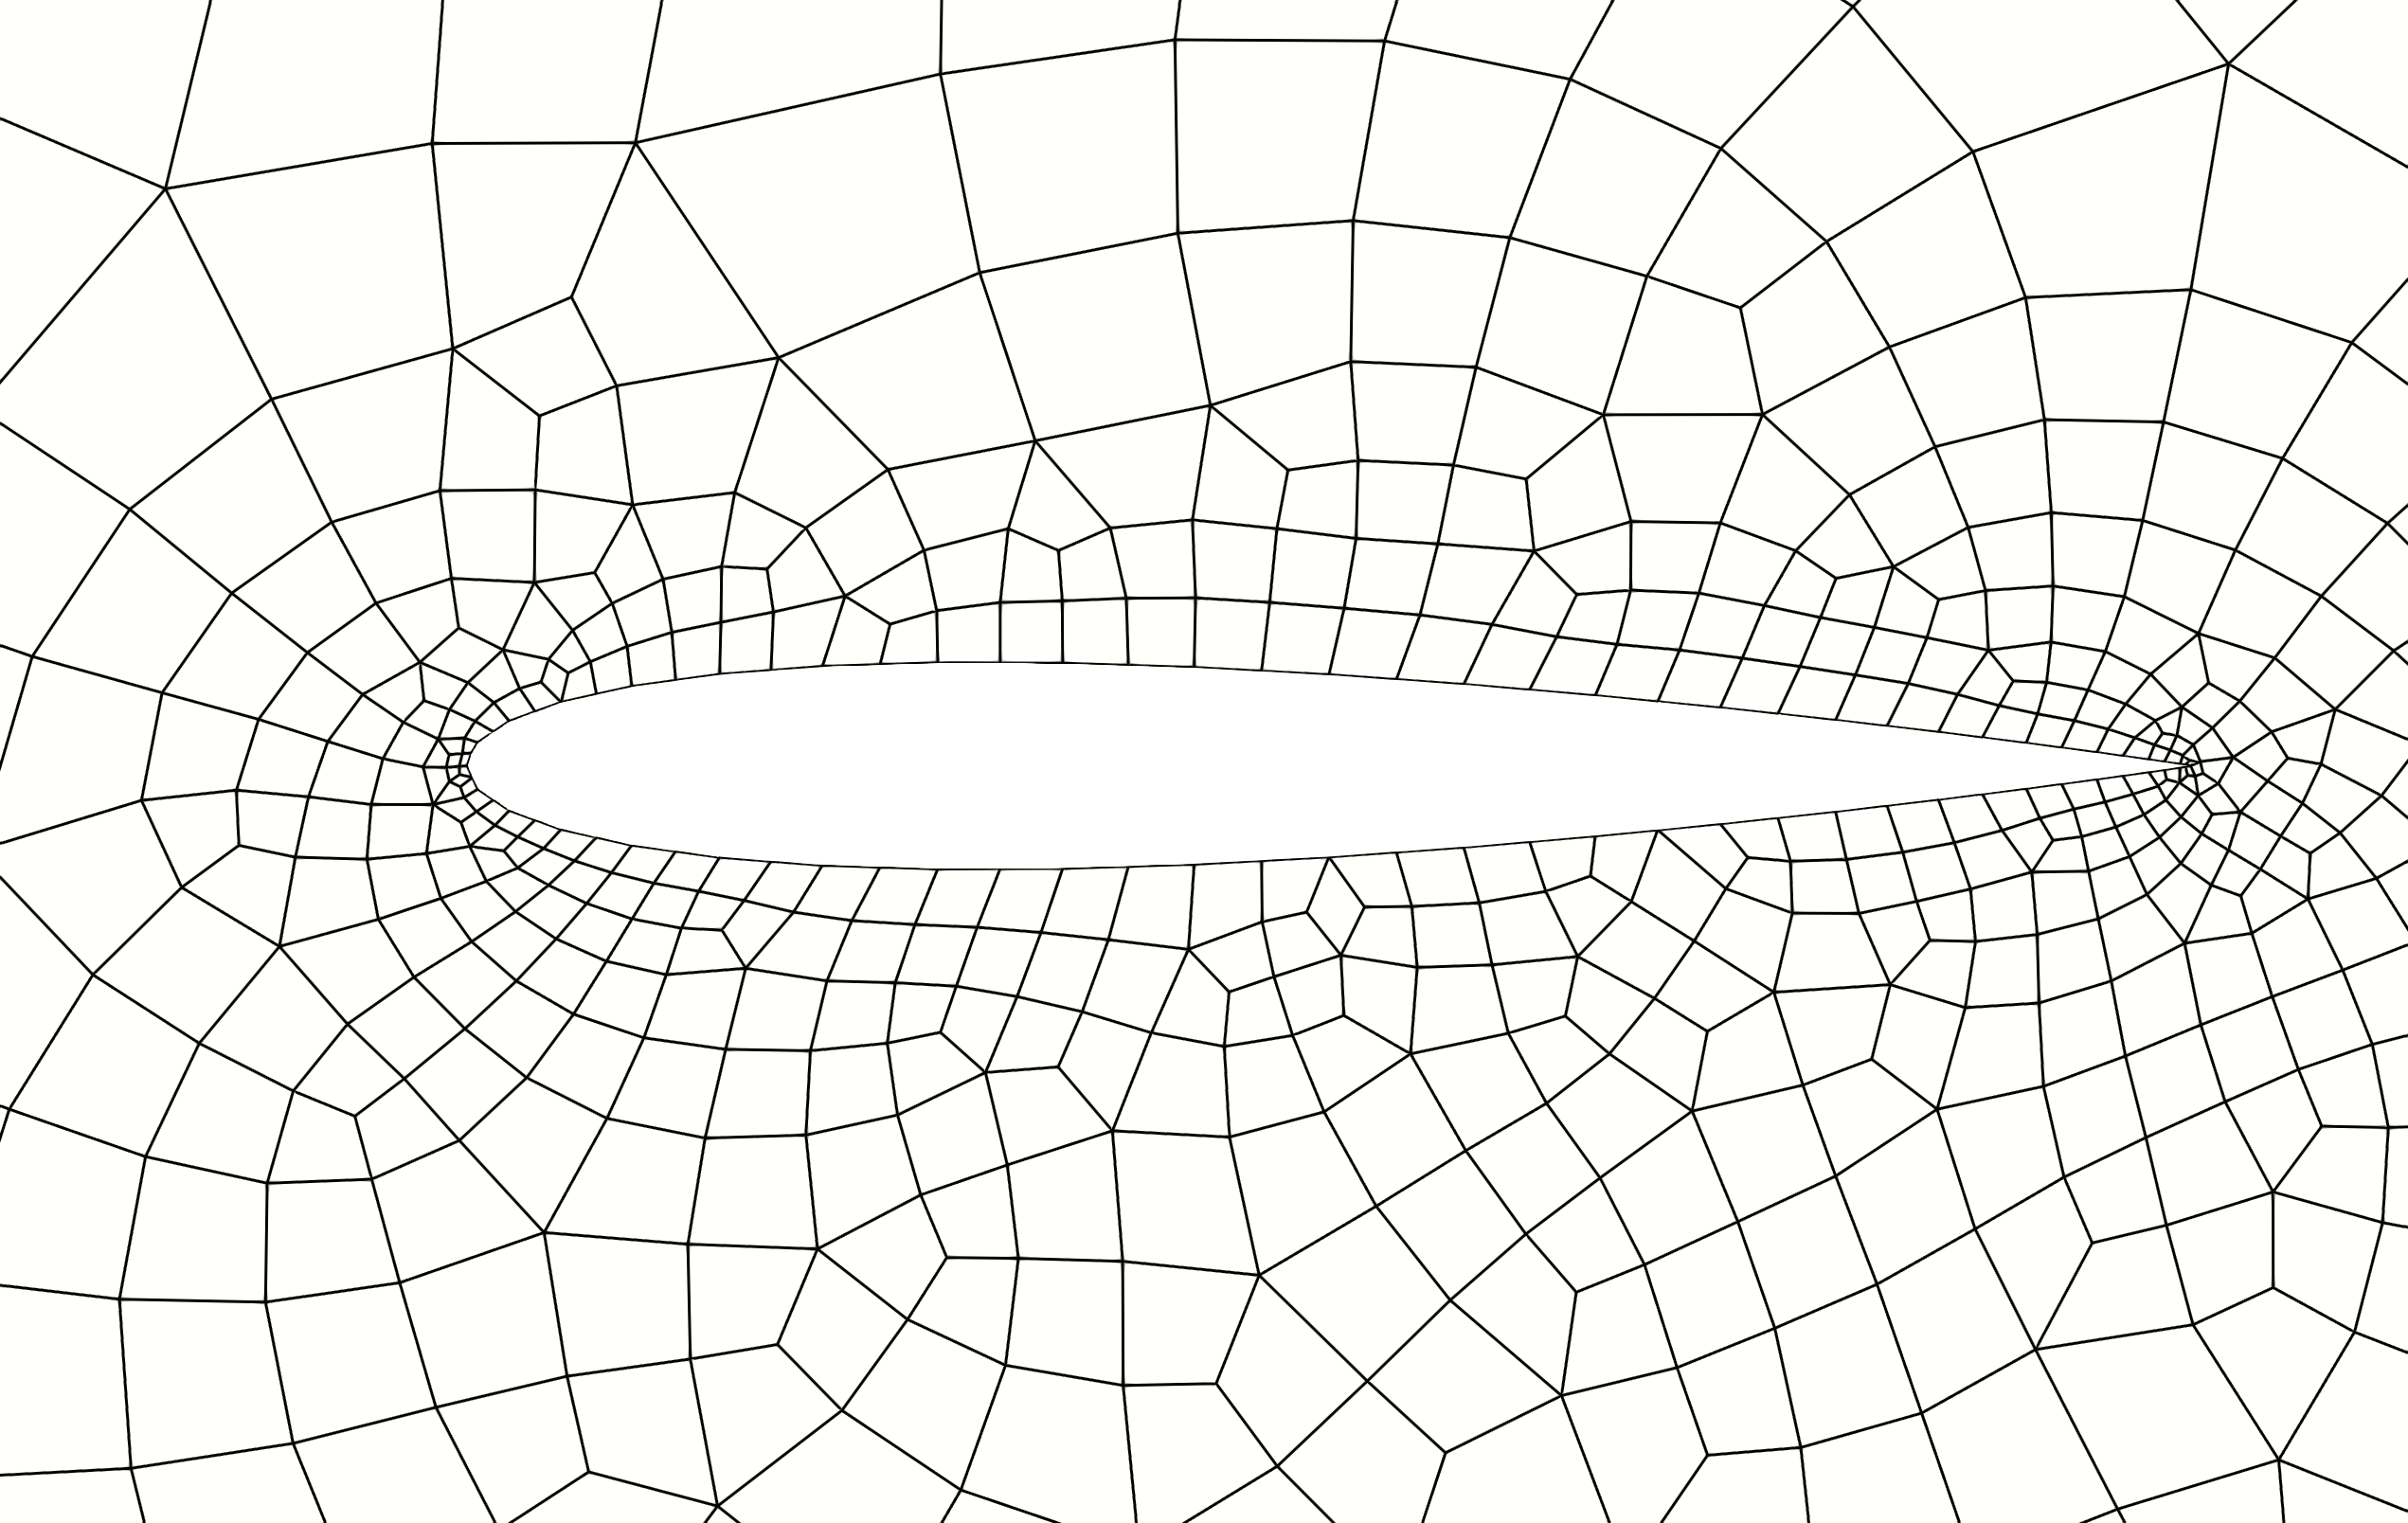
\includegraphics[width=0.45\textwidth]{Chapter_graphics_processing_units/media/unstructured_mesh}\label{fig:unstructured_mesh}}
    \caption{Types of meshes: (a) Structured (reprinted from~\cite{Rahman2015}) (b) Unstructured}\label{fig:mesh_types}
\end{figure}

Here a concession has been made for flexibility, as structured meshes would be faster than
unstructured meshes on a \acrshort{acr:GPU}. Threads on a \acrshort{acr:GPU} benefit from accessing
memory in an ordered fashion. With a structured mesh, thread warps need only one memory access to
obtain all their neighbours. As shown in Figure~\ref{fig:structured_memory}, the neighbours are
packed in memory, and their index can be computed easily by incrementing the element indices. For
unstructured meshes, neighbour indices have to be fetched from an area in memory, and the neighbours
are not guaranteed to be contiguous in memory. This adds an indirection, and may require multiple
memory accesses. Figure~\ref{fig:unstructured_memory} shows the relation between elements from an
unstructured mesh and their neighbours. Since unstructured meshes enable more complex meshes to be
represented than strictly regular quadrilaterals, this tradeoff is accepted, and acts as a worst
case scenario for the performance of \acrshortpl{acr:GPU}.

\begin{figure}[H]
    \centering
    \subfloat[Structured mesh]
    {\includesvg[height=0.32\textwidth]{Chapter_graphics_processing_units/media/structured_memory}\label{fig:structured_memory}}
    \hfill
    \subfloat[Unstructured mesh]
    {\includesvg[height=0.32\textwidth]{Chapter_graphics_processing_units/media/unstructured_memory}\label{fig:unstructured_memory}}
    \caption{Memory accesses: (a) Structured (b) Unstructured}\label{fig:mesh_memory}
\end{figure}

The program uses the \textit{\acrfull{acr:CGNS}} mesh format. Both the provided mesh generator and
mesh partitioner output the format, and the mesh partitioner and solver can read the format. The
format is widely used, which should enable this program to read the many meshes already available
using the format.

The program outputs data using the \textit{\acrfull{acr:VTK}} format. Once again, this is a widely
used format, notably used by the \textit{ParaView} visualisation application. The results of the
program should then be easy to manipulate and display.

\subsection{Ease of programming}\label{subsection:graphics_processing_units:data_structure:ease_of_programming}

The program is written partly using the object-oriented paradigm, especially for the data structure
part. Elements, faces and nodes are objects, each with multiple data members and member functions.
This groups many parameters together that would be separate arrays otherwise, making it easier to
program and keep track of the different members of objects. This has the disadvantage of putting
more pressure on the limited cache of \acrshortpl{acr:GPU} and of potentially increasing the number
of memory accesses needed. This is the structure of arrays vs array of structures debate. It
increases cache pressure when a loop only accesses a subset of the data members of an object. For
example, the solution update function only uses the solution and derivative of an element. When
threads loop over those elements, they have to load entire elements into cache. If the solution and
derivative were stored into separate arrays, many more elements could fit in cache as only their
solution and derivative would be fetched. This would also improve memory accesses, as warps of
threads would need fewer memory accesses since the data is continuous.

On the other hand, using objects simplifies many parts of the code. Elements can be sent and
received from process to process as a whole: adding a data member does not necessarily mean
modifying every part of the code that copies or creates elements. This is especially useful as we
can use constructors and destructors for objects.
On the other hand, using objects simplifies many parts of the code. Elements can be sent and
received from process to process as a whole: adding a data member does not necessarily mean
modifying every part of the code that copies or creates elements. This is especially useful as we
can use constructors and destructors for objects.

Constructors and destructors are used here because the objects use dynamic memory for their solution
data. As elements and faces can have a different polynomial order, they need to store more or less
data depending on the polynomial order. This makes it impossible to create an array of objects,
unless all objects use the maximum size they can have, negating the memory advantage of lower-order
elements. Instead, in this work objects use dynamic memory to hold their variable size arrays. They
hold pointers to that memory, making the objects themselves fixed in size. This has the added
benefit of making the objects smaller and easier to move around, as only the pointers and the
geometry data have to be moved while the bigger solution data stays in dynamic memory.
Figure~\ref{fig:moving_elements} shows how an element is moved from the sixth position of an array
to the fifth of another. Only the data contained directly in the element object is copied, while the
bulk of its data, the yellow pressure solution array in the case of the wave equation solver, stays
in place in dynamic memory. The green arrow represents the element being moved, and the red arrows
represent pointers.

\begin{figure}[H]
    \centering
    \includesvg[width=0.65\textwidth]{Chapter_graphics_processing_units/media/moving_elements}
    \caption{Moving elements: The data stored in dynamic memory does not need to be copied}\label{fig:moving_elements}
\end{figure}

Unlike the main arrays which are allocated from the \acrshort{acr:CPU} on the \acrshort{acr:GPU}
using the \acrshort{acr:CUDA} runtime, \acrshort{acr:GPU} dynamic memory is allocated on the
\acrshort{acr:GPU} itself. When the elements are created in a kernel, each thread allocates memory
in parallel in the object constructor. That memory is deallocated when the element is deleted.
Coupled with move semantics of modern C++, this allows an automatic management of that memory on the
\acrshort{acr:GPU}, similar to how we would use smart pointers or arrays in usual C++. Dynamic
memory allocation on the \acrshort{acr:GPU} is a relatively new feature, which enables programming
patterns closer to those used for \acrshort{acr:CPU} programming.

\section{Implementation}\label{section:graphics_processing_units:implementation}

\subsection{Memory transfers}\label{subsection:graphics_processing_units:implementation:memory}

\Acrshort{acr:GPU} memory is separate from \acrshort{acr:CPU} memory. In this work, we allocate
memory on the \acrshortpl{acr:GPU} in two ways: memory is allocated using the \acrshort{acr:CUDA}
runtime from the \acrshort{acr:CPU}, and memory is allocated in the \acrshort{acr:GPU} dynamic heap
directly from the \acrshort{acr:GPU}.

Memory allocated by the \acrshort{acr:CUDA} runtime can be transferred directly to and from the
\acrshort{acr:GPU}. We use it to manage arrays of high-level objects, such as elements, faces, and
nodes. These allocations and transfers can be performed asynchronously using execution
\textit{streams}. When using streams, operations are queued by the \acrshort{acr:CPU} for
asynchronous execution on the \acrshort{acr:GPU}. The \acrshort{acr:CPU} is then free to continue
executing the program. The \acrshort{acr:CPU} will only wait for the \acrshort{acr:GPU} to finish
execution if a non-asynchronous function is added to the stream, or we issue an explicit
synchronisation instruction such as \textit{cudaStreamSynchronize}. The \acrshort{acr:CPU} then
waits until all operations queued on the stream are completed on the \acrshort{acr:GPU}. The results
can then be used on the \acrshort{acr:CPU}.

Algorithm~\ref{alg:cuda_memory} shows how we would use that kind of memory. After creating our
execution stream, we allocate and fill a pressure solution array on the \acrshort{acr:CPU} as usual.
We then allocate an array on the \acrshort{acr:GPU}, and copy the data from the \acrshort{acr:CPU}
array to it. We can then perform computations on the \acrshort{acr:GPU} using that array with the
\textit{perform\_gpu\_computations} kernel. Kernels are explained in
Subsection~\ref{subsection:graphics_processing_units:implementation:kernels}. We can then copy back
the data from the \acrshort{acr:GPU} array to the \acrshort{acr:CPU} array using
\textit{cudaMemcpyAsync}. We synchronise with the execution stream to ensure the data has finished
copying, at which point we can use the \acrshort{acr:CPU} array. To finish up, we deallocate the
\acrshort{acr:CPU} array, the \acrshort{acr:GPU} array, and the execution stream.

\begin{algorithm}[H]
    \begin{cuda}
        auto main(int argc, char* argv[]) -> int {
            cudaStream_t stream;
            cudaStreamCreate(&stream); 

            const size_t length = 1000;
            double* pressure_cpu = new double[length];
            for (size_t i = 0; i < length; ++i){
                pressure_cpu[i] = 1.0;
            }
            double* pressure_gpu = nullptr;

            cudaMallocAsync(&pressure_gpu, length * sizeof(double), stream);
            cudaMemcpyAsync(pressure_gpu, pressure_cpu, length * sizeof(double), 
                cudaMemcpyHostToDevice, stream);

            const numBlocks = 10;
            const blockSize = 100;
            perform_gpu_computations<<<numBlocks, blockSize, 0, stream>>>(
            length, pressure_gpu);

            cudaMemcpyAsync(pressure_cpu, pressure_gpu, length * sizeof(double), 
                cudaMemcpyDeviceToHost, stream);
            cudaStreamSynchronize(stream);

            display_cpu_results(length, pressure_cpu);

            delete[] pressure_cpu;
            cudaFreeAsync(pressure_gpu, stream);
            cudaStreamDestroy(stream);
            return 0;
        }\end{cuda}
\caption{\textbf{cuda\_memory:} A pressure solution array is allocated on the \acrshort{acr:CPU}, then transferred back and forth to the \acrshort{acr:GPU}.}\label{alg:cuda_memory}
\end{algorithm}

Since dealing with pointers directly can become error-prone in larger programs, we encapsulate that
behaviour into a vector type. Algorithm~\ref{alg:device_vector} shows a simplified version of
Algorithm~\ref{alg:cuda_memory} using this new type.

\begin{algorithm}[H]
    \begin{cuda}
        using SEM::Device::Entities::device_vector;

        auto main(int argc, char* argv[]) -> int {
            cudaStream_t stream;
            cudaStreamCreate(&stream); 

            std::vector<double> pressure_cpu(1000, 1.0);
            device_vector<double> pressure_gpu(pressure_cpu, stream);

            const numBlocks = 10;
            const blockSize = 100;
            perform_gpu_computations<<<numBlocks, blockSize, 0, stream>>>(
                pressure_gpu.size(), pressure_gpu.data());
            
            pressure_gpu.copy_to(pressure_cpu, stream);
            cudaStreamSynchronize(stream);

            display_cpu_results(pressure_cpu);

            cudaStreamDestroy(stream);
            return 0;
        }\end{cuda}
\caption{\textbf{device\_vector:} A pressure solution vector is allocated on the \acrshort{acr:CPU}, then transferred back and forth to the \acrshort{acr:GPU}.}\label{alg:device_vector}
\end{algorithm}

Memory allocated in the \acrshort{acr:GPU} dynamic heap from the \acrshort{acr:GPU} is allocated by
the \textit{new} or \textit{malloc} functions similarly to how we would normally do this on the
\acrshort{acr:CPU}, but from the \acrshort{acr:GPU} using \acrshort{acr:GPU} functions like kernels.
We encapsulate these operations into \textit{cuda\_vector}, another vector type similar to that of
Algorithm~\ref{alg:device_vector}.

Memory from \acrshort{acr:GPU} heap cannot be transferred directly to the \acrshort{acr:CPU} using
\acrshort{acr:CUDA} functions like \textit{cudaMemcpyAsync}, as heap memory is not mapped to the
\acrshort{acr:CUDA} runtime. To transfer data from that kind of memory, we must copy it to a
\acrshort{acr:CUDA} runtime allocated array on the \acrshort{acr:GPU} using a kernel.

We use heap memory for dynamic data structures living on the \acrshort{acr:GPU} that the
\acrshort{acr:CPU} does not need to use, like the variably-sized solution arrays of individual
elements and faces, and the variably-sized lists of faces connected to an element's sides.

\subsection{Kernels}\label{subsection:graphics_processing_units:implementation:kernels}

Functions launched from regular \acrshort{acr:CPU} code and executing on the \acrshort{acr:GPU} are
called \textit{kernels}. Once a kernel is launched it is queued to be asynchronously executed on the
\acrshort{acr:GPU}. The \acrshort{acr:CPU} is then free to continue executing instructions. These
kernels, like memory transfers, are queued using execution streams.

Algorithms~\ref{alg:cuda_memory} and~\ref{alg:device_vector} show a kernel being launched, with an
array of pressure and its size as arguments. Two other interesting elements are the
\textit{numBlocks} and \textit{blockSize} parameters. These two parameters are used between angled
brackets \textbf{<\negmedspace<\negmedspace<\thickspace>\negmedspace>\negmedspace>} to
configure the kernel launch. They represent the number of blocks of threads and the number of
threads in a block, respectively. As described in
Subsection~\ref{subsection:graphics_processing_units:architecture:programming_model}, this dictates
how the kernel executes in parallel.

Algorithm~\ref{alg:perform_gpu_computations} shows the anatomy of a kernel, as well as a device
function. Kernels are annotated with \textbf{\_ \_global\_ \_}, and device functions with
\textbf{\_ \_device\_ \_}. Device functions are regular functions compiled to be called from the
\acrshort{acr:GPU}. The topology of the parallel work grid is stored in the \textit{gridDim} and
\textit{blockDim} variables, and the various indices of the threads are stored in the
\textit{blockIdx} and \textit{threadIdx} variables.

\begin{algorithm}[H]
    \begin{cuda}
        __device__ 
        auto get_pressure(double p, size_t i) -> double {
            return std::pow(p, i);
        }

        __global__
        auto perform_gpu_computations(size_t n, double* pressure) -> void {
            const int index = blockIdx.x * blockDim.x + threadIdx.x;
            const int stride = blockDim.x * gridDim.x;

            for (size_t i = index; i < n; i += stride) {
                pressure[i] = get_pressure(pressure[i], i);
            }
        }\end{cuda}
\caption{\textbf{perform\_gpu\_computations:} Computations are performed in parallel on the \acrshort{acr:GPU}.}\label{alg:perform_gpu_computations}
\end{algorithm}

\subsection{Parallel reductions}\label{subsection:graphics_processing_units:implementation:reductions}

Parallel reductions are operations that are difficult to make efficient on \acrshortpl{acr:GPU} and
saturate them with work. Harris et al.~\cite{Harris2007} show a few different ways to optimise these
operations. In this work, we need to compute the minimum time step over the whole mesh at every time
step. This operation uses geometric and solution data from the elements to find each element's
minimum time step size. This data is only available on the \acrshort{acr:GPU}. 

An implementation must saturate the \acrshort{acr:GPU} with work as much as possible: blindly
looping one thread over the whole mesh will only use one of the approximately five thousand cores of
the \acrshort{acr:GPU}, for one thousandth of the speed. Algorithm~\ref{alg:reduce_wave_delta_t}
shows how the \(\Delta t\) is computed in parallel over all the elements of a mesh. It implements
several of the optimisations from~\cite{Harris2007}.

\begin{algorithm}[H]
    \begin{cuda}
        template <unsigned int blockSize>
        __device__ 
        auto warp_reduce_delta_t_2D(volatile deviceFloat *sdata, unsigned int tid) -> void {
            if (blockSize >= 32) sdata[tid] = std::min(sdata[tid], sdata[tid + 16]);
            if (blockSize >= 16) sdata[tid] = std::min(sdata[tid], sdata[tid + 8]);
            if (blockSize >= 8) sdata[tid] = std::min(sdata[tid], sdata[tid + 4]);
            if (blockSize >= 4) sdata[tid] = std::min(sdata[tid], sdata[tid + 2]);
            if (blockSize >= 2) sdata[tid] = std::min(sdata[tid], sdata[tid + 1]);
        }

        template <unsigned int blockSize>
        __global__ 
        auto reduce_wave_delta_t(
                deviceFloat CFL, 
                size_t N_elements, 
                const Element2D_t* elements, 
                deviceFloat *g_odata) -> void {

            __shared__ deviceFloat sdata[(blockSize >= 64) ? blockSize: blockSize+blockSize/2];
            unsigned int tid = threadIdx.x;
            size_t i = blockIdx.x*(blockSize*2) + tid;
            unsigned int gridSize = blockSize*2*gridDim.x;
            sdata[tid] = std::numeric_limits<deviceFloat>::infinity();

            while (i < N_elements) { 
                deviceFloat delta_t_wave = 
                CFL * elements[i].delta_xy_min_
                    /(elements[i].N_ * elements[i].N_ * Constants::c);

                if (i+blockSize < N_elements) {
                    delta_t_wave = std::min(
                        delta_t_wave, 
                        CFL * elements[i+blockSize].delta_xy_min_
                            /(elements[i+blockSize].N_ * elements[i+blockSize].N_ * Constants::c));
                }

                sdata[tid] = std::min(sdata[tid], delta_t_wave); 
                i += gridSize; 
            }
            __syncthreads();

            if (blockSize >= 1024) { 
                if (tid < 512) { sdata[tid] = std::min(sdata[tid], sdata[tid + 512]); } 
                __syncthreads(); 
            }
            if (blockSize >= 512) { 
                if (tid < 256) { sdata[tid] = std::min(sdata[tid], sdata[tid + 256]); } 
                __syncthreads(); 
            }
            if (blockSize >= 256) { 
                if (tid < 128) { sdata[tid] = std::min(sdata[tid], sdata[tid + 128]); }
                __syncthreads(); 
            }
            if (blockSize >= 128) { 
                if (tid < 64) { sdata[tid] = std::min(sdata[tid], sdata[tid + 64]); } 
                __syncthreads(); 
            }

            if (tid < 32) warp_reduce_delta_t_2D<blockSize>(sdata, tid);
            if (tid == 0) g_odata[blockIdx.x] = sdata[0];
        }\end{cuda}
\caption{\textbf{reduce\_wave\_delta\_t:} The minimum \(\Delta t\) of the mesh is reduced in parallel.}\label{alg:reduce_wave_delta_t}
\end{algorithm}

Algorithm~\ref{alg:reduce_wave_delta_t} implements several advanced \acrshort{acr:CUDA} features not
discussed previously. The gist of it is that the threads from a block allocate a working array
\textit{sdata} in shared memory. That memory is local to a block of threads, and cannot be accessed
within other blocks. The threads then perform several reduction steps, where threads take the
minimum of two values with fewer and fewer threads active. Figure~\ref{fig:reduction} shows how
these steps are performed, with initially four threads active. Once there are \(32\) threads left, a
warp reduction function is called. This is necessary to remove branching within a warp. All threads
will execute these instructions, with threads that are not needed operating on useless data. Once
this is done, the first thread copies the result into the output array \textit{g\_odata}. There will
be one result per block of threads, the final step of the reduction will be performed on the
\acrshort{acr:CPU}. The function is templated on the size of the thread blocks. All the apparent
branching based on \textit{blockSize} will disappear when compiled, as the code is generated for a
specific \textit{blockSize}.

\begin{figure}[H]
    \centering
    \includesvg[width=0.45\textwidth]{Chapter_graphics_processing_units/media/reduction}
    \caption{Reduction: A block of threads computes the minimum of data}\label{fig:reduction}
\end{figure}

\subsection{MPI transfers}\label{subsection:graphics_processing_units:implementation:mpi_transfers}

The fact that the solution data resides on the \acrshort{acr:GPU} complicates transfers between the
different parallel workers. This is because only \acrshortpl{acr:CPU} can communicate with each
other over \acrshort{acr:MPI}. Solution data therefore needs to be fetched from the
\acrshort{acr:GPU} to the \acrshort{acr:CPU}, transferred between \acrshortpl{acr:CPU}, then
transferred from the receiving \acrshort{acr:CPU} to its \acrshort{acr:GPU}. This is compounded by
the fact that elements can have a different polynomial order \(N\) which changes the size of their
solution arrays, and that these solution arrays are stored in \acrshort{acr:GPU} heap memory.

Algorithm~\ref{alg:boundary_conditions} displays a simplified version of the \acrshort{acr:MPI}
transfers necessary at each time step to update the solution at boundaries between
\acrshortpl{acr:GPU}. This increased cost compared to traditional \acrshort{acr:CPU} versions of
these algorithms highlights the need to minimise the surface area between \acrshortpl{acr:GPU}, as
described in Chapter~\ref{chapter:load_balancing}. Note that variables ending with an underscore are
data members of the mesh object.

\begin{algorithm}[H]
    \begin{cuda}
        auto boundary_conditions() -> void {
            int global_rank;
            MPI_Comm_rank(MPI_COMM_WORLD, &global_rank);
            int global_size;
            MPI_Comm_size(MPI_COMM_WORLD, &global_size);

            get_MPI_interfaces<<<mpi_outgoing_numBlocks_, mpi_blockSize_, 0, stream_>>>(
                mpi_origin_.size(), elements_.data(), 
                mpi_origin_.data(), mpi_origin_side_.data(), max_N_, 
                device_p_.data(), device_u_.data(), device_v_.data());

            device_p_.copy_to(host_p_, stream_);
            device_u_.copy_to(host_u_, stream_);
            device_v_.copy_to(host_v_, stream_);
            cudaStreamSynchronize(stream_);
            
            for (size_t i = 0; i < mpi_process_.size(); ++i) {
                MPI_Isend(
                    host_p_.data() + mpi_outgoing_offset_[i] * (max_N_ + 1), 
                    mpi_outgoing_size_[i] * (max_N_ + 1), 
                    MPI_DOUBLE, mpi_process_[i], /*[...]*/);
                MPI_Irecv(
                    host_receiving_p_.data() + mpi_incoming_offset_[i] * (max_N_ + 1), 
                    mpi_incoming_size_[i] * (max_N_ + 1), 
                    MPI_DOUBLE, mpi_process_[i], /*[...]*/);

                MPI_Isend(
                    host_u_.data() + mpi_outgoing_offset_[i] * (max_N_ + 1), 
                    mpi_outgoing_size_[i] * (max_N_ + 1), 
                    MPI_DOUBLE, mpi_process_[i], /*[...]*/);
                MPI_Irecv(
                    host_receiving_u_.data() + mpi_incoming_offset_[i] * (max_N_ + 1), 
                    mpi_incoming_size_[i] * (max_N_ + 1), 
                    MPI_DOUBLE, mpi_process_[i], /*[...]*/);

                MPI_Isend(
                    host_v_.data() + mpi_outgoing_offset_[i] * (max_N_ + 1), 
                    mpi_outgoing_size_[i] * (max_N_ + 1), 
                    MPI_DOUBLE, mpi_process_[i], /*[...]*/);
                MPI_Irecv(
                    host_receiving_v_.data() + mpi_incoming_offset_[i] * (max_N_ + 1), 
                    mpi_incoming_size_[i] * (max_N_ + 1), 
                    MPI_DOUBLE, mpi_process_[i], /*[...]*/);
            }

            MPI_Waitall(6 * mpi_process_.size(), requests_.data(), statuses_.data());

            device_receiving_p_.copy_from(host_receiving_p_, stream_);
            device_receiving_u_.copy_from(host_receiving_u_, stream_);
            device_receiving_v_.copy_from(host_receiving_v_, stream_);

            put_MPI_interfaces<<<mpi_incoming_numBlocks_, mpi_blockSize_, 0, stream_>>>(
                mpi_destination_.size(), elements_.data(), 
                mpi_destination_.data(), max_N_, 
                device_receiving_p_.data(), device_receiving_u_.data(), device_receiving_v_.data());
        }\end{cuda}
\caption{\textbf{boundary\_conditions:} The solution of elements on either side of the interface between \acrshortpl{acr:GPU} is transferred.}\label{alg:boundary_conditions}
\end{algorithm}